\documentclass[11pt,a4paper,oneside]{article}
\usepackage{longtable}
\usepackage{lscape}
\usepackage{graphicx}
\usepackage{amsfonts}
\usepackage{amsmath}
\usepackage{amsthm}
\usepackage{amssymb}
\usepackage{calc}
\usepackage[cp1252]{inputenc}
\usepackage[left=1.0in,right=1.5in,top=1.0in,bottom=1.0in,includeheadfoot]{geometry}
\usepackage{fancyhdr}
\usepackage{hyperref}
\usepackage{float}
\pagestyle{fancy}
\fancyhead[LO]{\nouppercase{\leftmark}}
\fancyhead[R]{\nouppercase{\rightmark}}
\fancyhead[RO]{\thepage}
\fancyfoot[LO]{\today}
\fancyfoot[C]{}
\fancyfoot[R]{FYS4150}
\renewcommand{\footrulewidth}{0.5 pt}
\setlength{\headheight}{16.0 pt}
\begin{document}
	\title{\textbf{\textbf{\Huge Project 5}}}
	\author{Jose Emilio Ruiz Navarro}
	\maketitle
	\begin{abstract}In this project, an molecular dynamics code is used to simulate a simple argon system and find the melting temperature using the measurements of the diffusion constant as a means to distinguish between the solid and liquid phases, with the value for the temperature being $~285$ K. Two different integrators, Euler-Cromer and Velocity-Verlet, were used to run the simulations and their energy performance was assessed for comparison. The results showed that the Velocity-Verlet integrator was much better than the Euler-Cromer by more than three orders of magnitude for small timesteps.\end{abstract}
	\newpage
	\tableofcontents
	\newpage
	
	\section{Introduction}
	
		All the files are located here: \url{https://github.com/jeruiznavarro/FYS3150/tree/master/Project5}.\\
	
		Molecular dynamics, or MD for short, is a computational technique that can be used to simulate particle systems that interact with each other by means of a \textit{classical} force field, which can take many forms and be used for many different systems. The main purpose of such a simulation is not to gain insights on the trajectories of the particles but to calculate equilibrium and transport properties in a large variety of materials and systems. This does not mean that it can't be used to see the trajectories of the particles in a system, but accuracy will be steadily lost as the simulation progresses because such systems are chaotic in nature, and thus extremely sensitive to the initial conditions, a tiny variation will yield totally different trajectories. Fortunately, this is not a problem when the objective is to measure some property where all (or at least a great majority) of the particles contribute in some way, like for example the diffusion coefficient. As long as the possible different microstates spawned by the variations in the initial conditions represent the same macrostate, the measurements won't be affected by this chaotic effect.\\
		
		MD was first described as a technique almost 60 years ago in 1957: "The method consists of solving exactly (to the number of significant figures carried) the simultaneous classical equations of motion of several hundred particles by means of fast electronic computors."\cite{alder} The simulations were run on an UNIVAC and an IBM-704 running programs written in machine code or FORTRAN I with up to $500$ hard sphere-like particles. Obviously everything has evolved a lot since then, but the core of this very basic idea remains intact, and the main differences are the increased complexity allowing to perform more advanced and varied tasks as well as how cheap and easy is to run these simulations today with much faster processors and ubiquitous access to parallel computing.\\
		
		The technique is quite popular in some biological fields like biophysics and biochemistry because it can offer insights into the structure of many important macromolecules, most notably proteins and nucleic acids (DNA and RNA) among others. The topic of protein folding sees extensive use of MD and improvements on it could lead to great medical advances. There are also studies in other biological structures like membranes/layers or even small viruses\cite{virus}. For similar reasons, it can be used in chemistry and physics (mainly statistical and solid state physics) to study complex molecules like fullerenes, to probe into transport phenomena (like diffusion in this work or adsorption), structural properties like the radial distribution function or defects, processes in solids like fracture and friction, etc. It is an important tool\\
		
		There are obviously a few limitations to MD. As previously stated, the systems that can be modelled using the paradigms of the technique are chaotic, so this can make things complicated if the system is especially sensitive (for example if they are small). There's also the problem of ergodicity, since time averaging is so important to obtain results a non ergodic system will be "unsolvable" under a MD scheme. It should be kept in mind that the most crucial part of the simulation is the interaction between the particles, without the appropriate force fields/potentials the results will be bad in the best possible case. Time and size are important constraints, without massively parallel computational power, a decently sized system can only be simulated for relatively short time scales in the order of the nanoseconds. Finally, everything is treated in a strictly classical approach, thus no quantum effects must be relevant in the systems to be simulated, like high frequency hydrogen bonds for example.\\
		 	
	\section{Theory and methods}
	
		There are two key parts behind the theory of MD, the force field and the integration. The first one is quite simple in this case since a suitable potential is available. The second one is also very simple but somewhat trickier.\\
		
		The potential that will be used is the standard Lennard-Jones potential that works on a pair of particles:\\
		
		\begin{equation*}U\left(r_{ij}\right)=4\epsilon\left[\left(\frac{\sigma}{r_{ij}}\right)^{12}-\left(\frac{\sigma}{r_{ij}}\right)^6\right]=4\epsilon\left(\frac{\sigma}{r_{ij}}\right)^6\left[\left(\frac{\sigma}{r_{ij}}\right)^6-1\right]\end{equation*}\\
		
		Where $\epsilon$ gives the dimensions of energy and controls the depth of the well and $\sigma$ represents the point where $U\left(r_{ij}\right)=0$. The negative term is responsible for the long-range attraction and has a physical basis on the behaviour of dipoles, while the positive term accounts for the short-range repulsion and has an exponent equal to $12$ for convenience as seen by the factorisation, but it has no physical meaning beyond accounting for the repulsion (other values are possible too, $9$ is also used in some situations). Using this expression for the potential the force will be given by its negative gradient:\\
		
		\begin{equation*}\mathbf{F}\left(r_{ij}\right)=-\nabla_{ij}U\left(r_{ij}\right)=-\frac{\partial U\left(r_{ij}\right)}{\partial r_{ij}}\nabla_{ij}\mathbf{r}_{ij}=24\epsilon\left(\frac{\sigma}{r_{ij}}\right)^6\left[2\left(\frac{\sigma}{r_{ij}}\right)^6-1\right]\frac{\mathbf{r}_{ij}}{r_{ij}^2}\end{equation*}\\
		
		Where $\nabla_{ij}$ acts on the coordinates of $x_{ij}$, $y_{ij}$ and $z_{ij}$. That is everything needed for the interaction part of the program, save for the effects introduced by the periodic boundary conditions. These boundary conditions must be used in the simulation to avoid surface effects being relevant. Considering the amount of particles that are found in the systems simulated with MD, $~\left(10^3,10^6\right)$ typically, between $10\%$ and $1\%$ of the particles will be in the surface. This can have very important implications because it is not a realistic circumstance, in real life atoms and molecules are usually grouped in much bigger associations than a few millions of atoms. For example it is critical to use them because the particles should not be bounded in their movement (they should not bounce on any limit) so that the diffusion process can take place normally with the particles being free to "travel" unobstructed as far as the dynamics of the system will take them. To implement these conditions it suffices to connect each face of the box in which the system is being simulated with the opposite one, so when a particle crosses on of the faces of said box it will appear on the opposite side, as if the system was a four dimensional torus. The minimum image convention (or cell lists) can be used so that there is no problem when the particles interact with those on the opposite side of the system.\\
		
		With the interactions set, now the integration must be taken care of. While equally simple to implement, there are a few more theoretical remarks. Two integrators are used in this work: Euler-Cromer and Velocity-Verlet. Actually, the only reason to use the Euler-Cromer integrator is to compare it with the Velocity-Verlet one which is much better (and is the default integrator for MD programs since it's simple and accurate). The Euler-Cromer integrator suffers from many ills, particularly a very bad energy conservation (having a high energy drift as time grows), it's not time reversible and is not area-preserving in the phase space. On the other hand, the Velocity-Verlet integrator does not have this problems and it is just a bit more complex than the Euler-Cromer integrator, so the choice is obvious. For reference, the Euler-Cromer integrator is defined by:\\
		
		\begin{equation*}\mathbf{v}\left(t+\Delta t\right)=\mathbf{v}\left(t\right)+\mathbf{a}\left(t\right)\Delta t\end{equation*}
		
		\begin{equation*}\mathbf{r}\left(t+\Delta t\right)=\mathbf{r}\left(t\right)+\mathbf{v}\left(t+\Delta t\right)\Delta t\end{equation*}\\
		
		While the Velocity-Verlet is defined by:\\
		
		\begin{equation*}\mathbf{v}\left(t+\Delta t/2\right)=\mathbf{v}\left(t\right)+\mathbf{a}\left(t\right)\frac{\Delta t}{2}\end{equation*}
		
		\begin{equation*}\mathbf{r}\left(t+\Delta t\right)=\mathbf{r}\left(t\right)+\mathbf{v}\left(t+\Delta t/2\right)\Delta t\end{equation*}
		
		\begin{equation*}\mathbf{v}\left(t+\Delta t\right)=\mathbf{v}\left(t+\Delta t/2\right)+\mathbf{a}\left(t+\Delta t\right)\frac{\Delta t}{2}\end{equation*}\\
		
		As for measurements, the temperature can be easily computed using the equipartition theorem:\\
		
		\begin{equation*}\left\langle E_k\right\rangle=\frac{3}{2}Nk_BT\hspace{0.25 cm}\Rightarrow\hspace{0.25 cm}T=\frac{2E_k}{3Nk_B}=\frac{\sum_{i=1}^N{m_iv_i^2}}{3Nk_B}\end{equation*}\\
		
		Where $N$ is the amount of atoms in the system. And to obtain the diffusion constant it suffices to calculate the mean square displacement defined as follows:\\
				
		\begin{equation*}\left\langle r^2\left(t\right)\right\rangle=6Dt\end{equation*}\\
		
		With $t$ being the time. For each individual atom it is defined as:\\
		
		\begin{equation*}r_i^2\left(t\right)=\left|\mathbf{r}_i\left(t\right)-\mathbf{r}_i\left(0\right)\right|^2\end{equation*}\\
		
		For more details about theoretical aspects of MD in general the following review\cite{understanding} and its subsequent references contain a lot of information with varying degrees of depth. And for the particular case of argon, this article\cite{argon}, while old, deals with the same issues presented in this work.\\
		
		For the code, the general structure that all MD codes follow is conceptually very simple and similar to how an actual experiment is performed.\\
		
		First of all, the program needs the initial conditions (parameters like pressure or temperature, positions, speeds, masses, etc.), these are usually read from file, but sometimes positions and speeds can be generated by some procedure, for example if the particles start in a crystalline lattice it's very easy to generate them at runtime.\\
		
		Next, the system is initialised (removing global momentum of the system, minimising high-energy configurations if needed, etc.) and the forces are calculated if they were not provided before (which is the most common case). Calculating the forces is by far the most intensive part of the simulation, it usually takes up more than half of the machine time during the run, this means that efforts on improving the computational efficiency must be focused on this part of the code.\\
		
		After the forces have been obtained, the integration of the movement can start, there are many algorithms to do this, each one with its weaknesses and strengths as it was previously discussed. This part is also intensive but not as much as the calculation of the forces because it scales as $\mathcal{O}\left(n\right)$ instead of $\mathcal{O}\left(n^2\right)$ like the force calculation.\\
		
		Finally, the appropriate measurements are taken if needed (most of the time is not interesting to take measurements on every single timestep). After this has been done, the next timestep starts and the program goes back to the force calculation until all the timesteps have been completed. Then it may be necessary to carry out some post-processing of the measurements before terminating the simulation depending on what was measured.\\
		
		To visualise this process in a better way, a flow chart is provided below:\\
		
		\begin{figure}[ht!]\begin{center}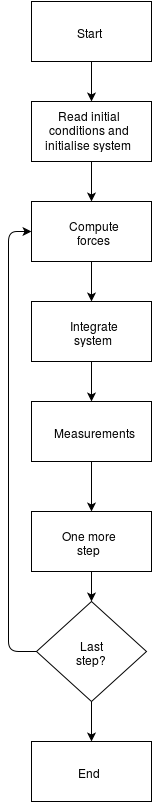
\includegraphics[scale=0.5]{MD.png}\par\protect\caption{\scriptsize General flow diagram of a molecular dynamics program.}\end{center}\end{figure}
		
	\section{Results}

		The measured density of the system was $~0.0275$ atoms per cubic \AA, which is equal to approximately $1.824$ times as dense as water, a reasonable value. This density only depends on the lattice constant used since the dimensions of the box size, the mass of the atoms or how many of them there are in the system are constants.\\
		
		To compare both integrators, it would be a good idea to see how the standard deviation of the total energy of the system behaves as a function of the timestep:\\
		
		\begin{figure}[ht!]\begin{center}\includegraphics[scale=1]{sigma_e.eps}\par\protect\caption{\scriptsize $\sigma_E$ vs. $\Delta t$ for the Euler-Cromer and the Velocity-Verlet integrators.}\end{center}\end{figure}
		
		The decrease in the temperature at the beginning is due to the exchange between kinetic energy and potential energy (which is quite precisely conserved by the Velocity-Verlet integrator) that takes place in the system. A perfect lattice is not a realistic initial condition, the system will be far away from the microstates to the initial total energy. This exchange between kinetic and potential energy is a result of this, as the system to become as stable as possible. It should also kept in mind that an MD algorithm minimises the potential energy and not the free energy, so there is an extra artificial reason for this phenomenon.\\
		
		The ratio between the initial temperature and the final equilibrium temperature is approximately below $1/2$, but it can be as small as $1/3$ depending on the initial conditions. This may be explained as a cause of particles getting very close to each other. Since the initial velocities are random according to Gaussian distribution centred in zero with a width that depends on the temperature, the higher the later is, the bigger the chances of having many particles with relatively high velocities, which would have the effect previously described. Especially because it is more common to find smaller ratios of temperatures the higher the initial one is.\\
		
		To estimate the melting temperature, the diffusion measurements can be used since the diffusion constant will be very small in the solid state:\newpage
		
		\begin{figure}[ht!]\begin{center}\includegraphics[scale=1]{diffusion.eps}\par\protect\caption{\scriptsize $D$ vs. $T$, the clear increase shows the system melting.}\end{center}\end{figure}
		
	\section{Conclusions}
	
		Looking at figure 2, it is obvious that the Velocity-Verlet integrator is the best one. For the smallest values of the timestep, the difference is about three orders of magnitude for the standard deviation of the total energy, and even for the highest timestep the difference is more than one order of magnitude, the Euler-Cromer integrator simply can't compete with it. The Velocity-Verlet could be worse than the Euler-Cromer if the tendencies shown in the plot are extrapolated, but this would not be a real problem since at such high timesteps the dynamics of the systems start being the main source of error since the characteristic time scales are comparable to the timestep. In such a situation, spurious effects introduced by the algorithm don't pose a problem since other tools should be used under those circumstances.\\
		
		In figure 3, it's very clear that there is a sharp increase in the value of the diffusion constant in a very small temperature interval. This allows for the estimation of the melting temperature of the system as it goes from solid to liquid. Since the increase is very sudden between $280$ and $290$ K, a tentative value of $285$ K is a reasonable choice. It is also remarkable that the values for the diffusion constant remain practically the same for a wide range of temperatures before the phase transition happens. This was expected, because the particles in a solid will oscillate around fixed equilibrium positions, even if the amplitude of the oscillations grows because the temperature becomes higher. It is not until the melting temperature is reached that there are visible changes in the diffusion constant.\\
	
		In the future, it would be interesting to try using a parallel approach to the program so that bigger systems could be simulated (or the same systems being simulated for a longer period of time). More complex schemes like cells list or neighbour lists could be used to improve the efficiency of the force calculation function of the program, which is the main bottleneck towards faster computation. Trying to use other force fields would enable the possibility of simulating molecules instead of simple atoms (although this requires a much more complex program). Finally, there are other physical properties of interest that could be measured without much effort, like pressure or the radial structure function.\\
	
		As for the didactic value of the project, I would personally say that it was a very valuable introduction to object orientated programming. Above the physical topics covered, I feel this is the most important lesson learnt in this case, because it provides a nice way to start learning how to deal with classes and objects in general. From a more physical point of view, it is a nice way to get a different view of statistical mechanics and thermodynamics in general, since it offers the possibility of "playing" with a system and "seeing" what happens with it constituent parts. It also exposes the student to some not-so-famous physical topics (compared to the Ising model or the initial numerical exercises) like the different integrators or the Lennard-Jones potential.\\
	
	\bibliographystyle{abbrv}
	\bibliography{bibliography.bib}
		
\end{document}